\begin{figure}[htpb]
	\centering\capstart{}
	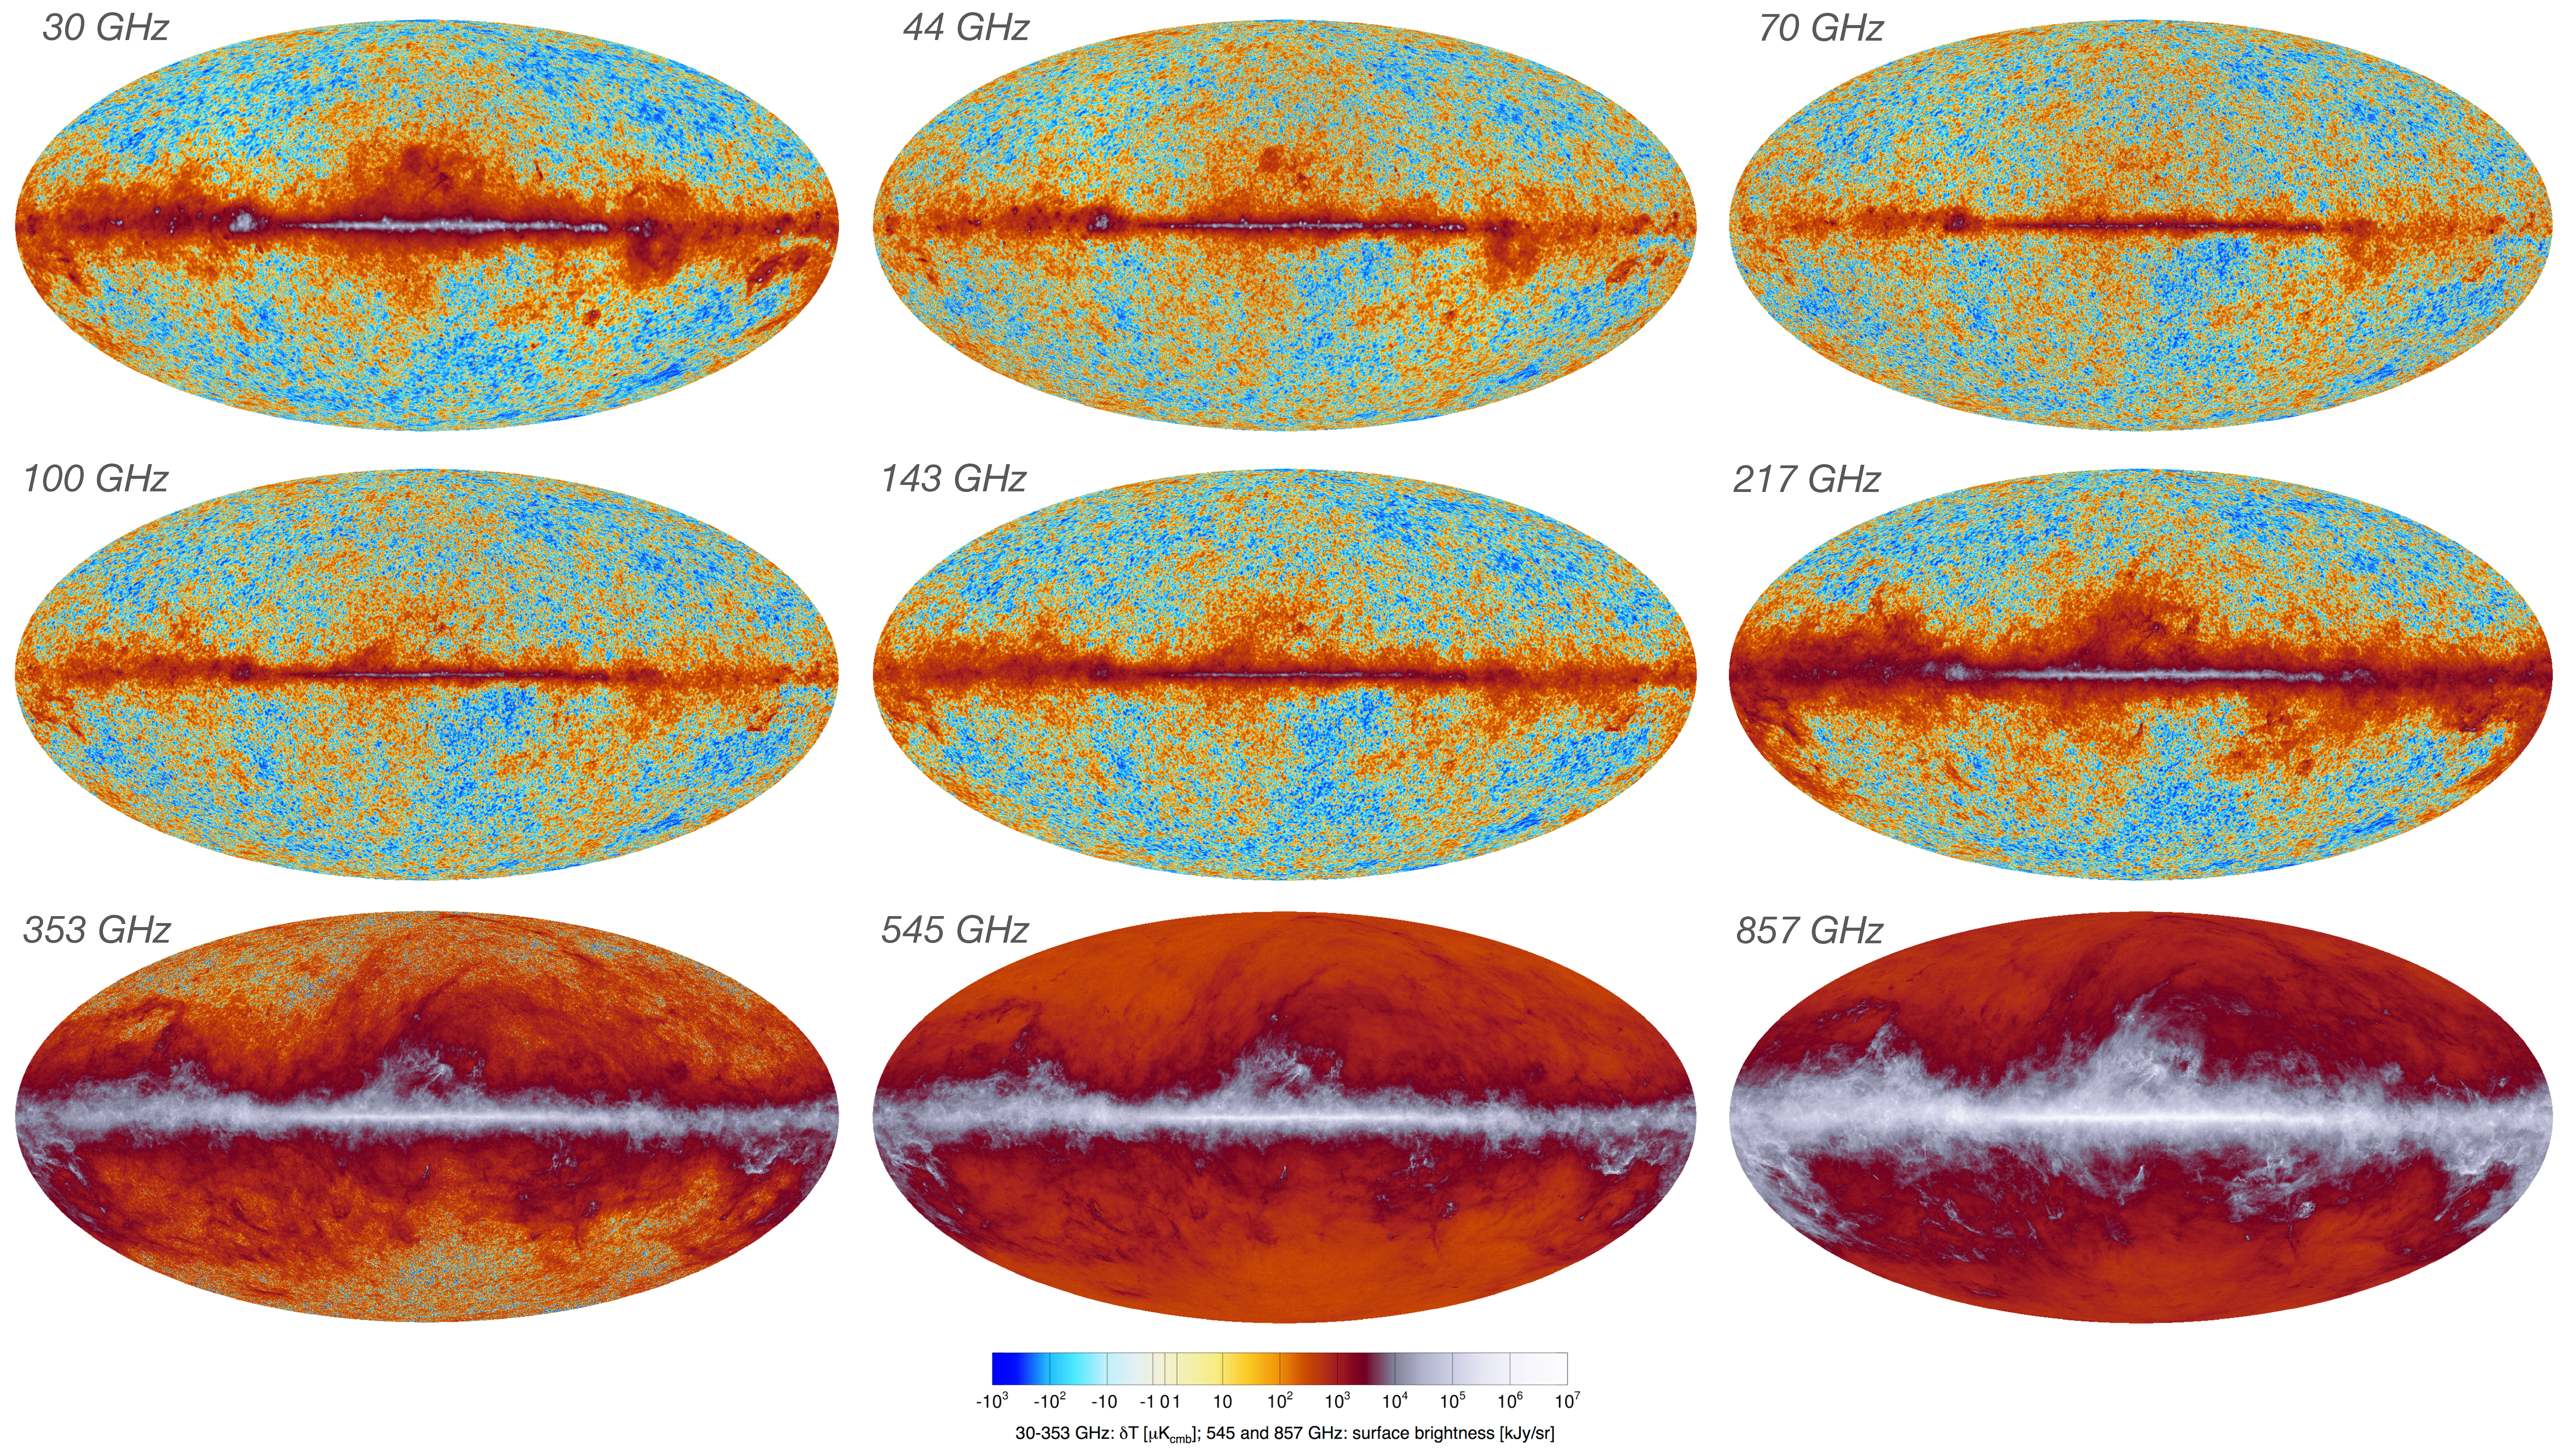
\includegraphics[trim={0 200 0 0},clip,width=\textwidth]{planck_2018_temp_freq.pdf}
	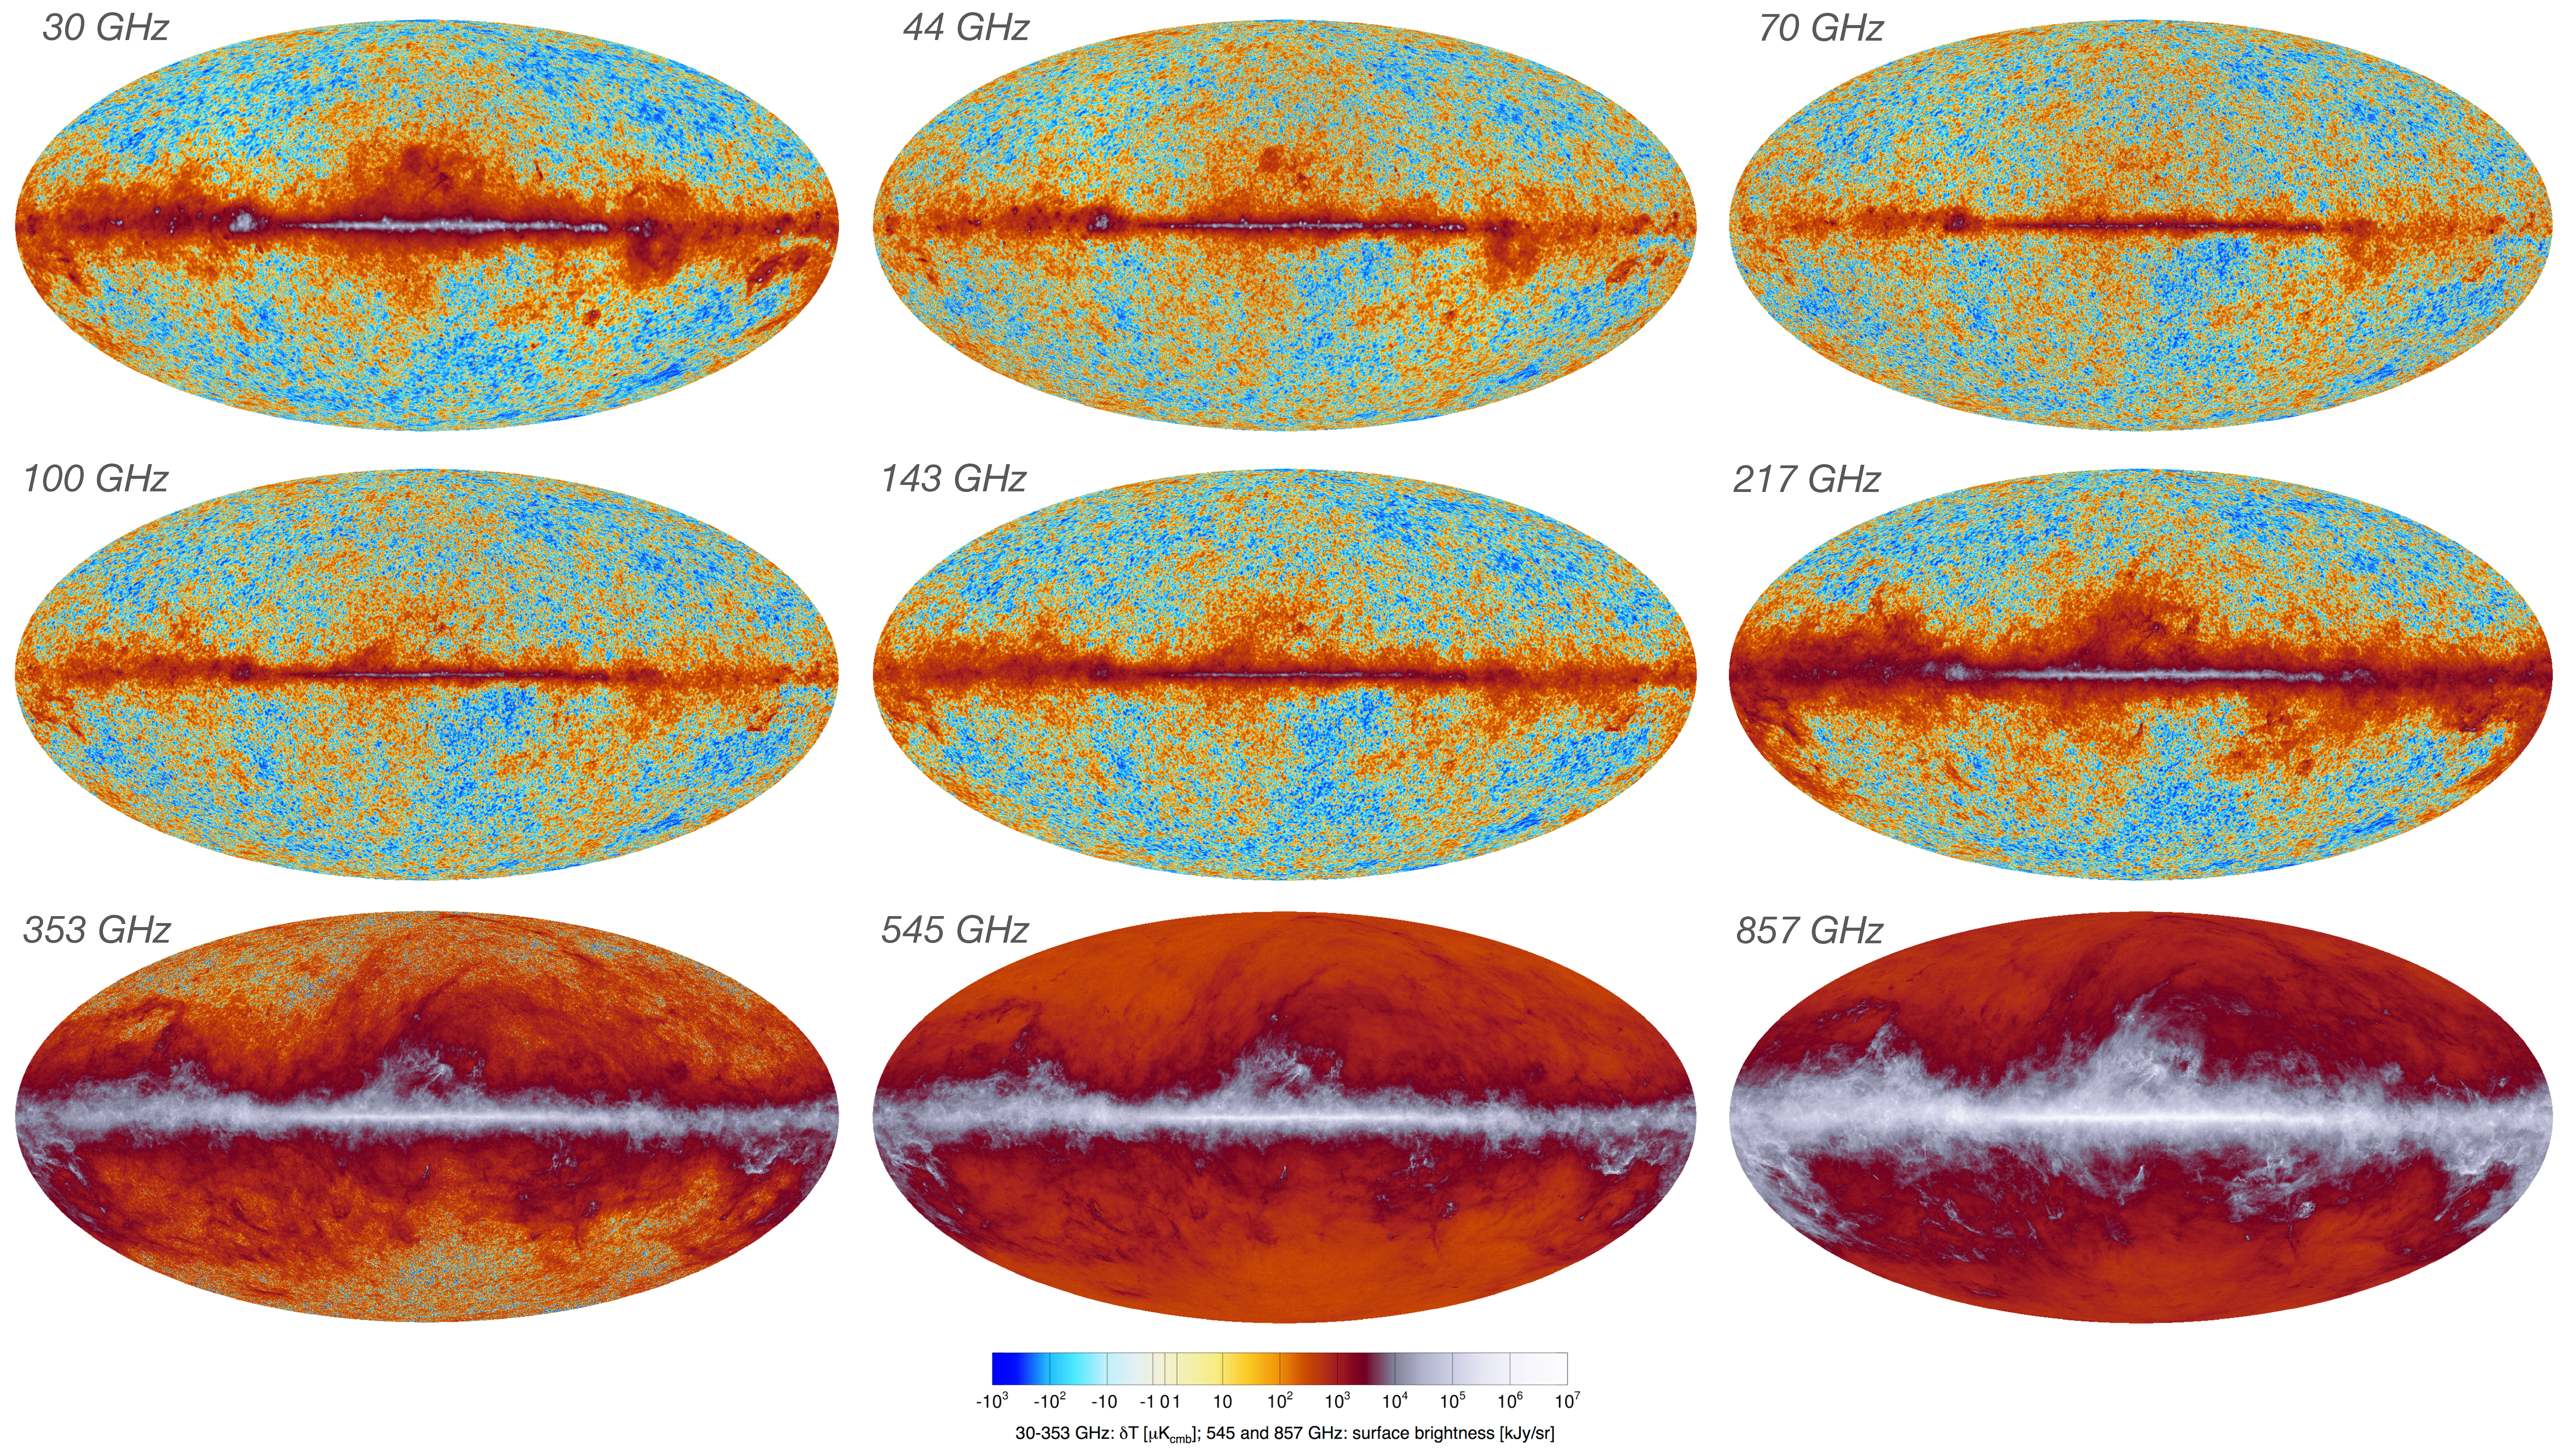
\includegraphics[trim={1000 0 1000 2100},clip,width=\textwidth]{planck_2018_temp_freq.pdf}
	\caption[
		The 2018 \emph{Planck} maps in intensity in each frequency band
	]{
		Fluctuations of sky emission in each of nine \emph{Planck} frequency bands, after removal of a common dipole component (courtesy of \emph{The Planck Collaboration 2018}~\cite{Planck2020}).
		Note that the CMB is obstructed by the foreground microwave emissions of the Milky Way at all frequencies.
	}\label{fig:chapter2_planck_frequency}
\end{figure}
